%ब 
\section{Insert} \label{s:results-insert}
% \newcommand{\Width}{0.5\textwidth}
% \newcommand{\TB}[1]{\textbf{#1}}
% An \texttt{insert} operation triggers a referential integrity validation
% whenever a child entity containing foreign keys is inserted where the
% \texttt{ValidationHandler} validates that the foreign keys exist as primary keys
% in the parent entities.
Across all the solutions in the experiments,  \texttt{insert}  triggers a
validation when \texttt{Enrolment} entities are inserted as it is a child entity
containing foreign keys of \texttt{Student} and \texttt{Course} entities.
\texttt{Student} and \texttt{Course} entities do not trigger validations as
these do not contain any references to other column families. 

The response time and throughput for completing an \texttt{insert} on a single
entity for all the solutions are presented in Figure~\ref{fres:Insert}.
Figure~\ref{fres:Insert-responsetime} shows the time consumed by each solution
to complete one \texttt{insert} operation in each of the three entities.
Figure~\ref{fres:Insert-throughput} shows the number of \texttt{insert}
operations that can be completed in one second across the solutions.

	\begin{figure}[H] 
		\subfigure[Response time for Insert operation]
		{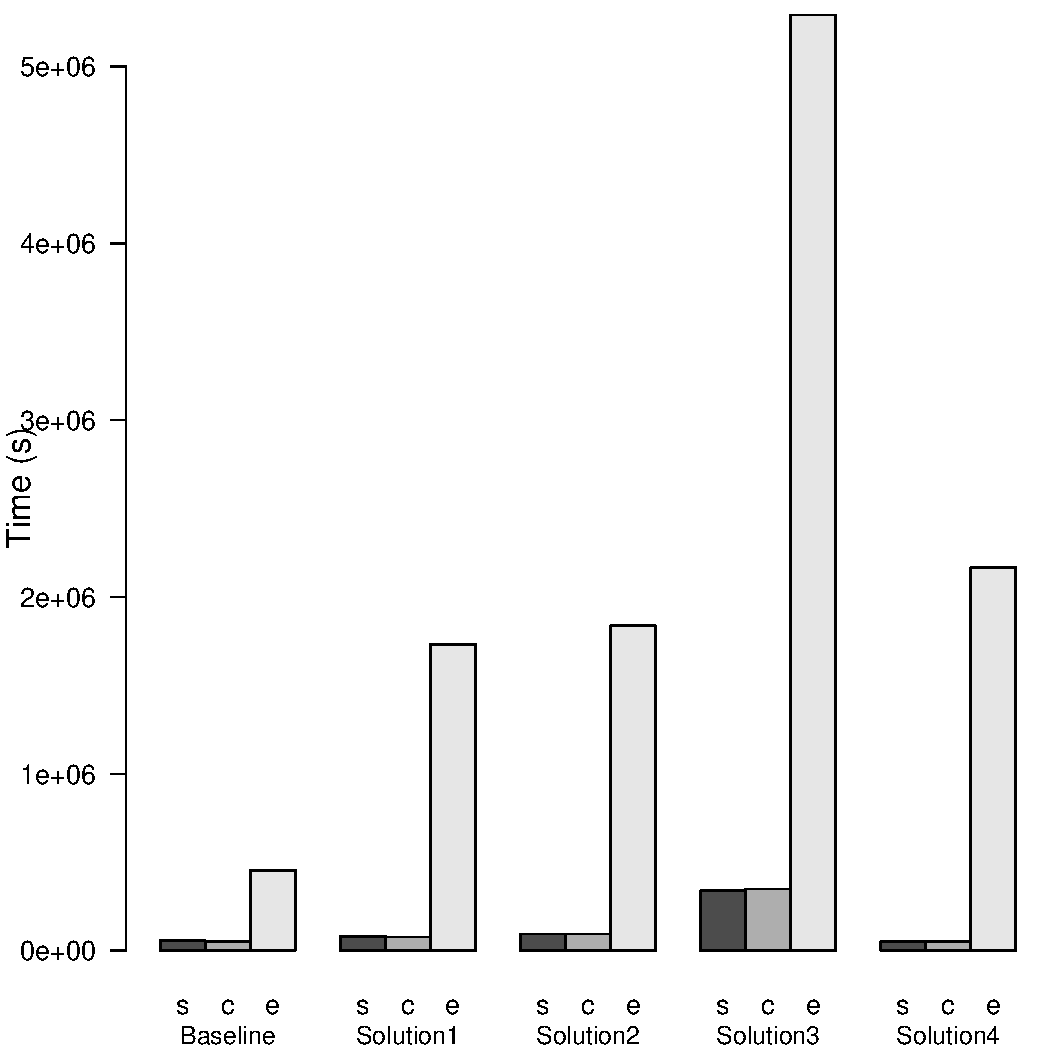
\includegraphics[width=\Width]{figure/result/barplot-insert-rt.pdf}\label{fres:Insert-responsetime}}
		\subfigure[Throughput for Insert operation]
		{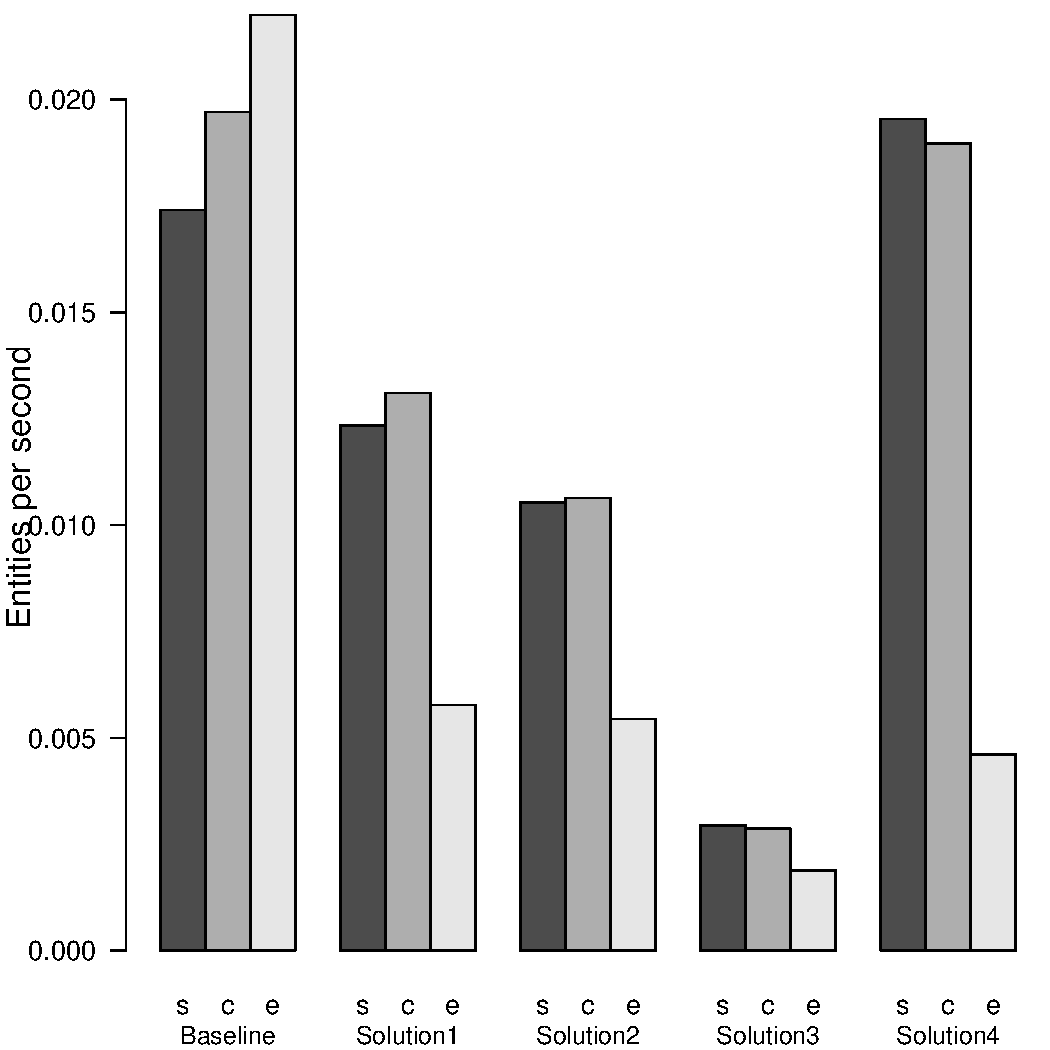
\includegraphics[width=\Width]{figure/result/barplot-insert-tp.pdf}\label{fres:Insert-throughput}}
		\caption{Performance of Solutions in Insert}\label{fres:Insert}
	\end{figure}
	
These results show
% and the results in Figures~\ref{fres:insert-user} and~\ref{fres:insert-course}
that \texttt{insert} on a single entity of \texttt{Student} and \texttt{Course}
take approximately the same time to complete. On the other hand, \texttt{insert}
on a single \texttt{Enrolment} entity takes the most time in all the solutions.
Inserting \texttt{Student} and \texttt{Course} entities into their respective
column families is fastest as these are parent column families and do not
trigger any validation. \texttt{insert} on these entities involves only
accessing its relevant \ac{FK} constraints from the metadata in order to
determine whether it is a parent or child entity. If the entity is a parent, the
validations are not triggered which is the case for \texttt{Student} and
\texttt{Course} entities. However, \texttt{Enrolment} entities have existing
\ac{FK} constraints indicating that they reference a parent entity which in turn
triggers referential integrity validations. Therefore,  its
validation involves not only identifying its relevant constraints but also
accessing its parent column families \texttt{Student} and \texttt{Course} to
ensure the existence of the foreign keys.
The results highlight the difference in response time when validation is
triggered in the case of \texttt{Enrolment} as well as when it is not initiated
in the parent entities.
% the validation of one \texttt{Enrolment} entity and for other entities that do
% not have validations.
Note that these observations stand true across all the solutions.

More information about the performance of each solution when an \texttt{insert}
operation is executed on each entity is presented in
Figures~\ref{fres:insert-user},~\ref{fres:insert-course}
and~\ref{fres:insert-enrolment}.
These figures show the response time for one \texttt{insert}
on all the three entities in every solution and the throughput for the
operations.
Figure~\ref{fres:insert-user} presents the results for \texttt{insert} on a
single \texttt{Student} entity in all the solutions. Similarly
Figures~\ref{fres:insert-course} and~\ref{fres:insert-enrolment} show the
performance of \texttt{insert} on a \texttt{Course} and \texttt{Enrolment}
entity in the solutions. It can be seen that Solution~4 takes the least time to
complete an \texttt{insert} on all the entities while Solution~3 takes the most
time. Both Solutions~1 and 2 perform similarly and are slightly slower than
Solution~4. These differences are because of the way their metadata is stored
and accessed as explained in Section~\ref{s:results-overview}.

When compared to the baseline, it is clear that the referential integrity
validations as well as metadata access caused the increased response time for
\texttt{insert} in all the solutions. Since the validations are the same for all
solutions, the performance differences in the solutions are due to the different
ways of accessing and processing the metadata.
Solution~4 is almost three times slower than the baseline to perform the
validations on \texttt{insert} while Solution~3 is more than eleven times
slower. Both Solutions~1 and 2 are almost four times slower than the baseline.
% Solution~3 takes the most time to perform one \texttt{insert} on all the
% entities.
However, when no validations are triggered Solution~4 performs almost similar to
the baseline while Solution~3 is still about two times slower than the baseline.
In this case, Solutions~1 and 2 are only about 0.5 times slower than the
baseline. Note that the time to \texttt{insert} \texttt{Student} and
\texttt{Course} entities in Baseline and Solution~4 are similar (Figures~\ref{fres:insert-user}
and~\ref{fres:insert-course}). A possible reason for this is that baseline
operations are affected by the initialization as its \texttt{insert} operations
are the very first operations to be executed.

\newpage
		\begin{figure}[H]
		\centering
		\newcommand{\W}{.4\textwidth}
			\subfigure[Response time for Insert on Student]
			{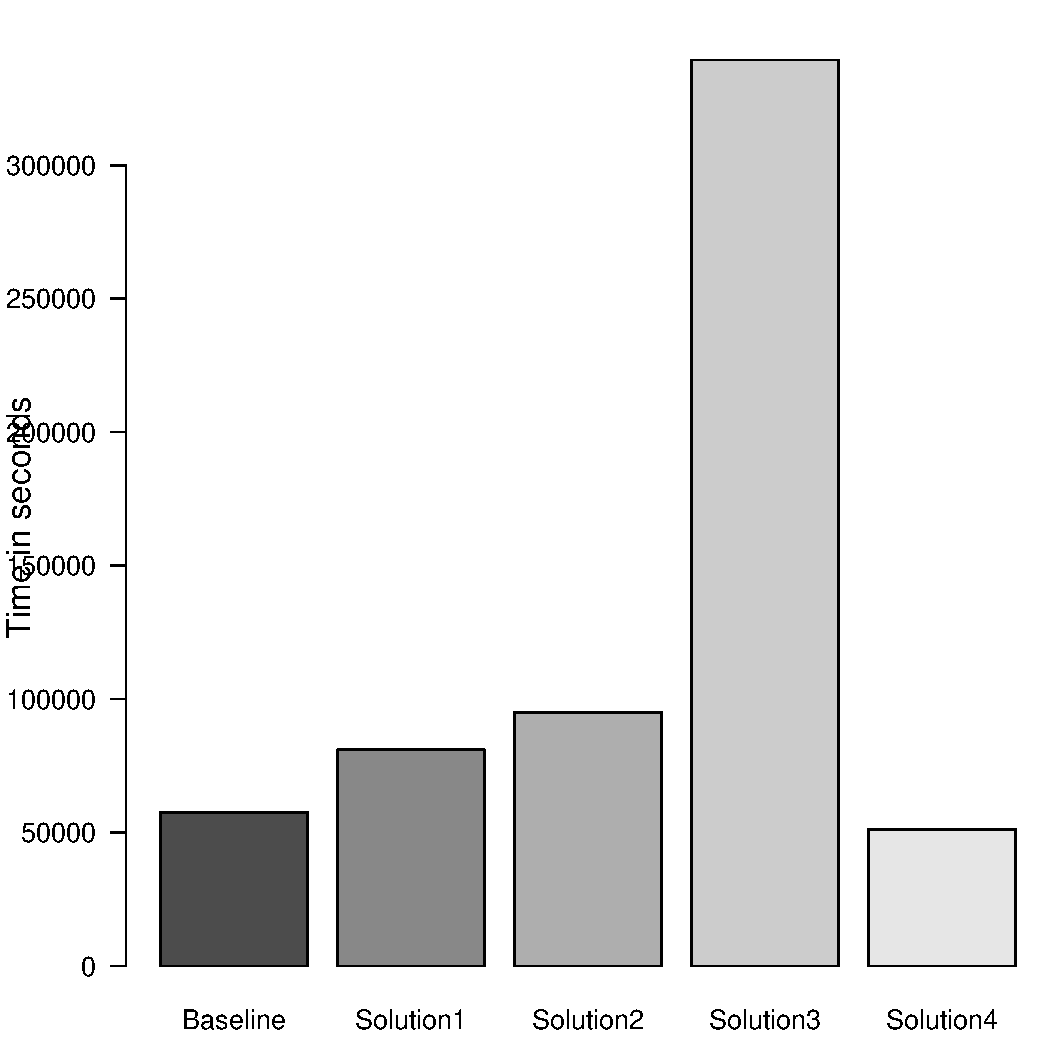
\includegraphics[width=\W]{figure/result/barplot-insert_student-rt.pdf}}
			\subfigure[Throughput for Insert on Student]
			{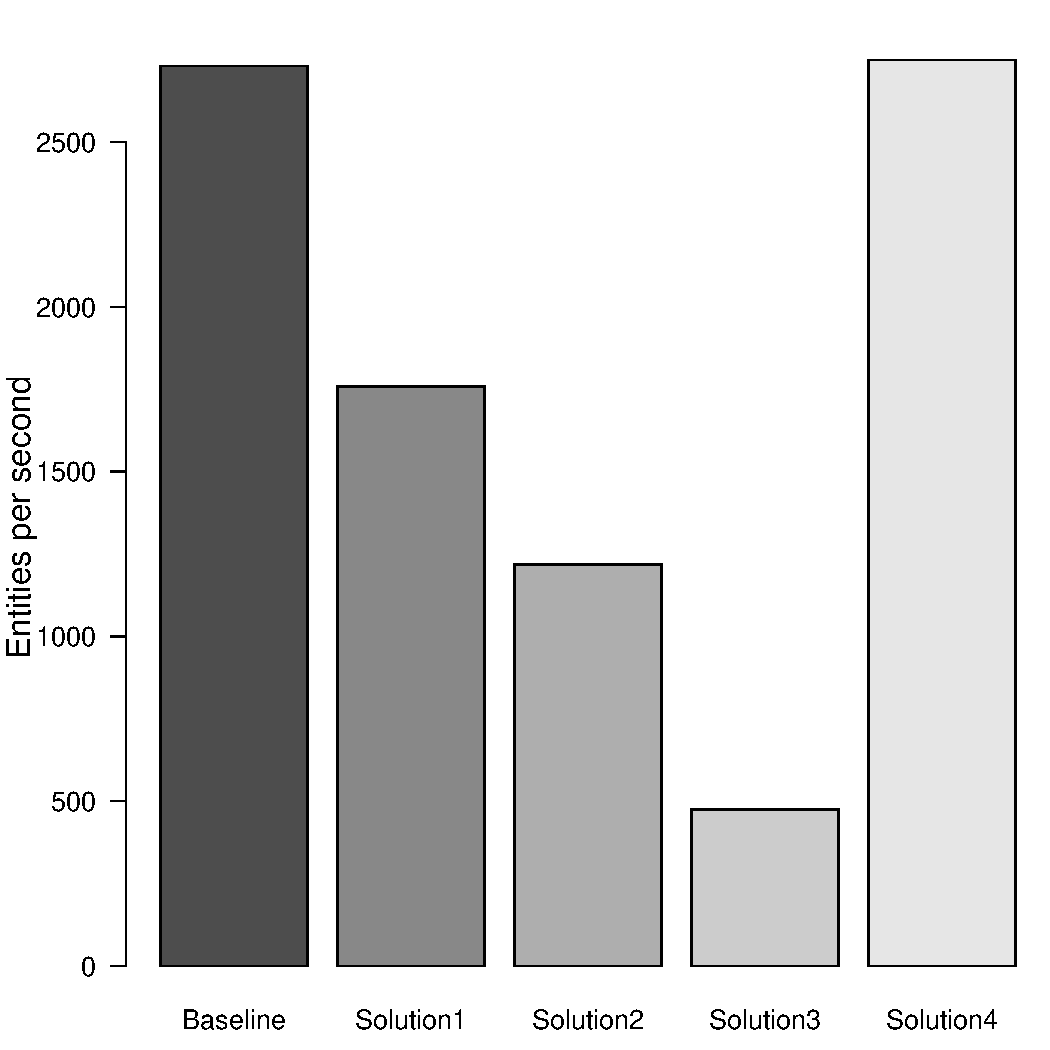
\includegraphics[width=\W]{figure/result/barplot-insert_student-tp.pdf}}
			\caption{Performance inserting students}\label{fres:insert-user}
% 		\end{figure}
% \newpage
% 	\subsection{Course}
% 		\begin{figure}[H]
			\subfigure[Response time for Insert on Course]
			{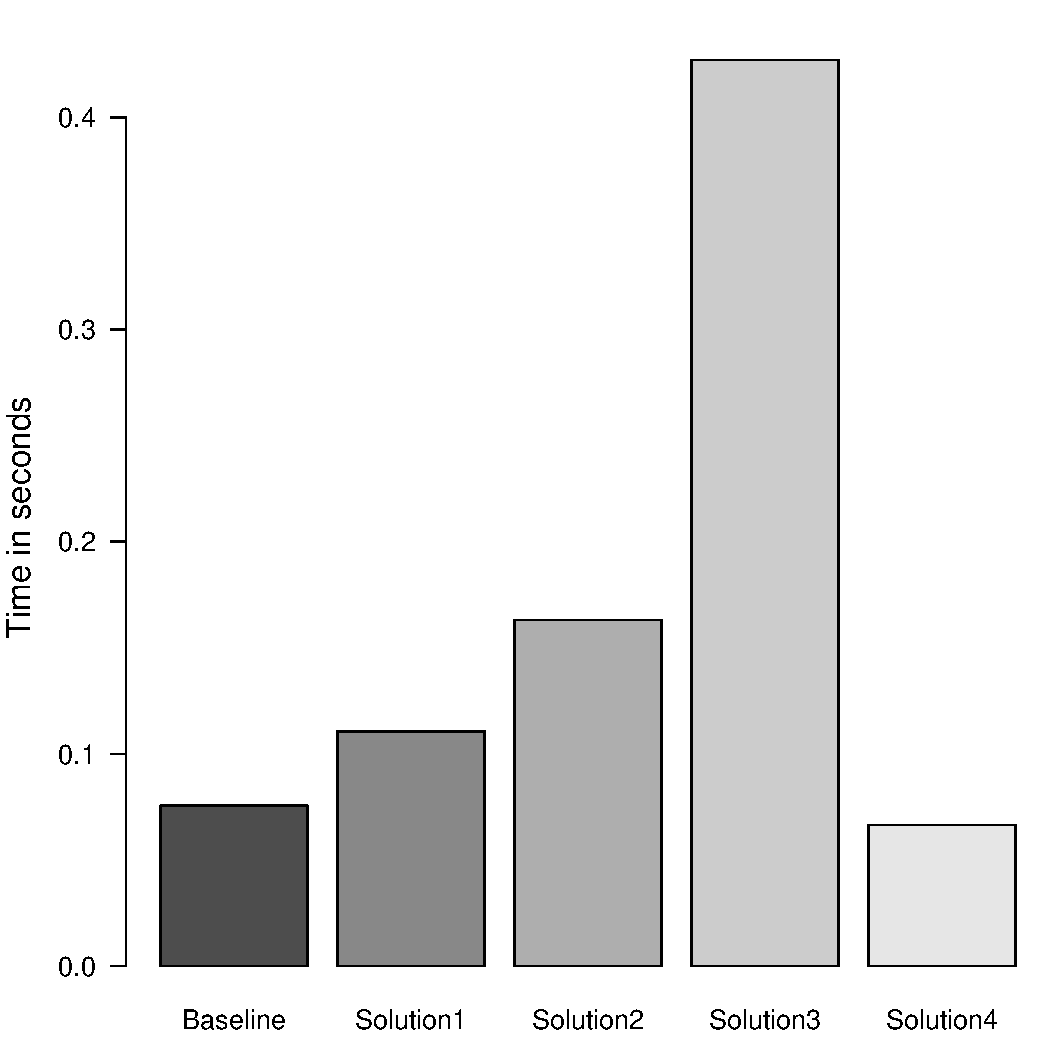
\includegraphics[width=\W]{figure/result/barplot-insert_course-rt.pdf}}
			\subfigure[Throughput for Insert on Course]
			{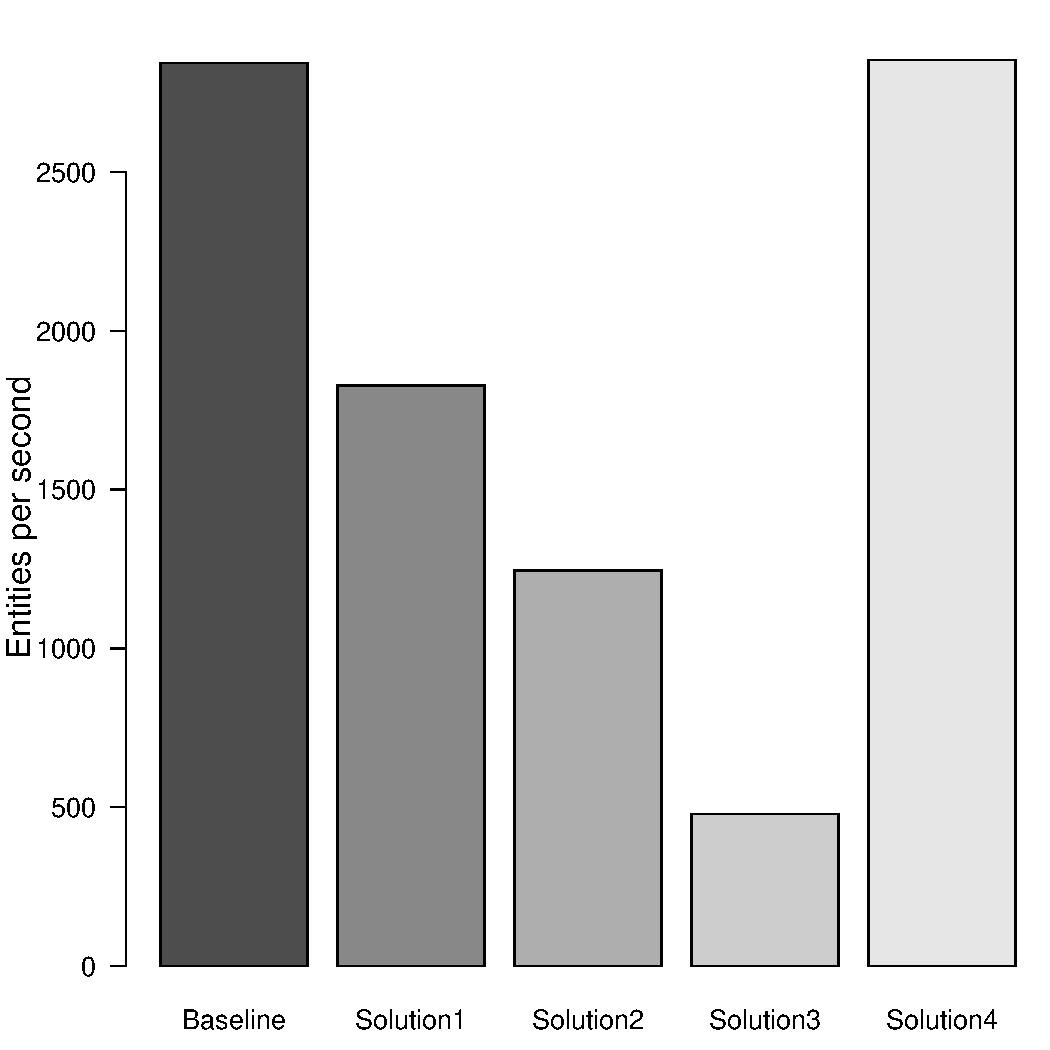
\includegraphics[width=\W]{figure/result/barplot-insert_course-tp.pdf}}
			\caption{Performance inserting courses}\label{fres:insert-course}
% 		\end{figure}
% \newpage
% 	\subsection{Enrolment}
% 		\begin{figure}[H]
			\subfigure[Response time for Insert on Enrolment]
			{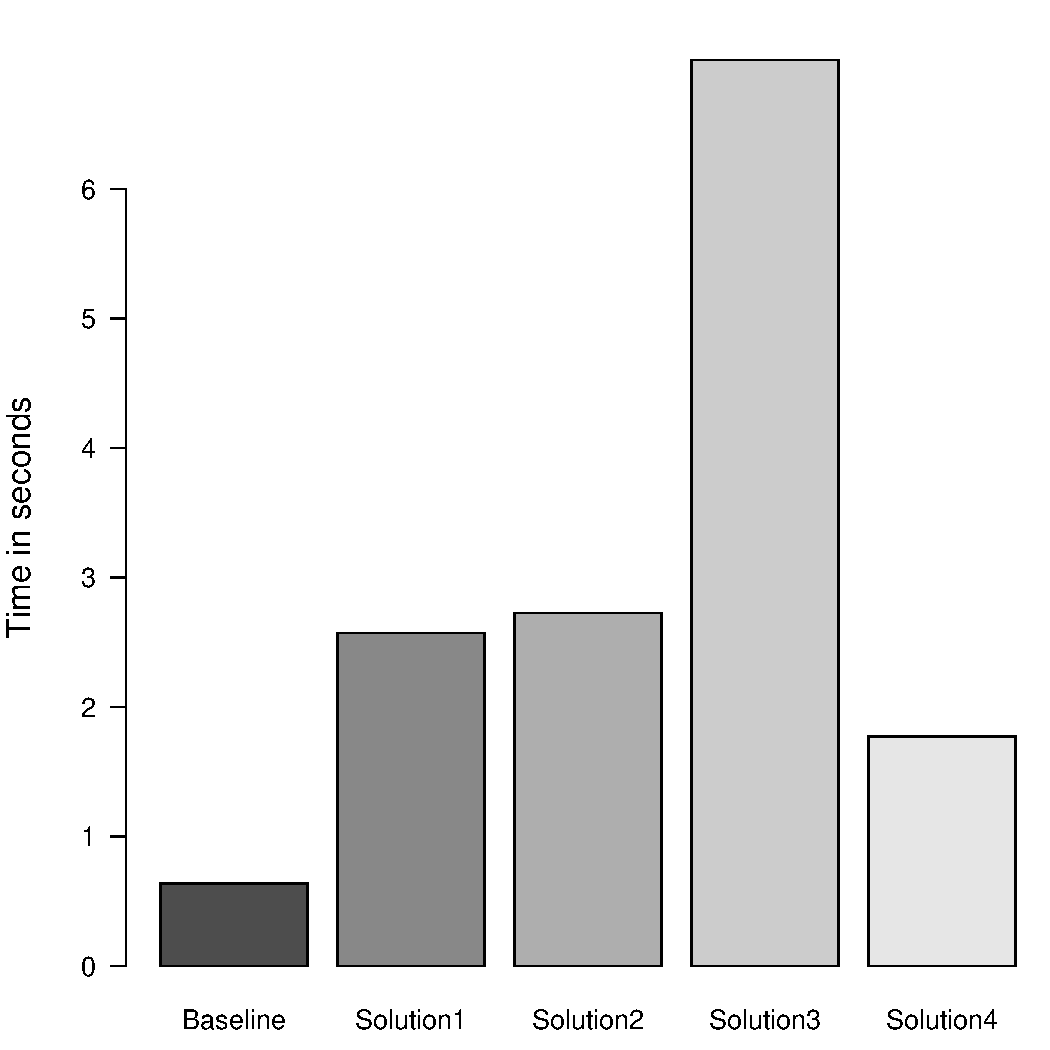
\includegraphics[width=\W]{figure/result/barplot-insert_enrolment-rt.pdf}}
			\subfigure[Throughput for Insert on Enrolment]
			{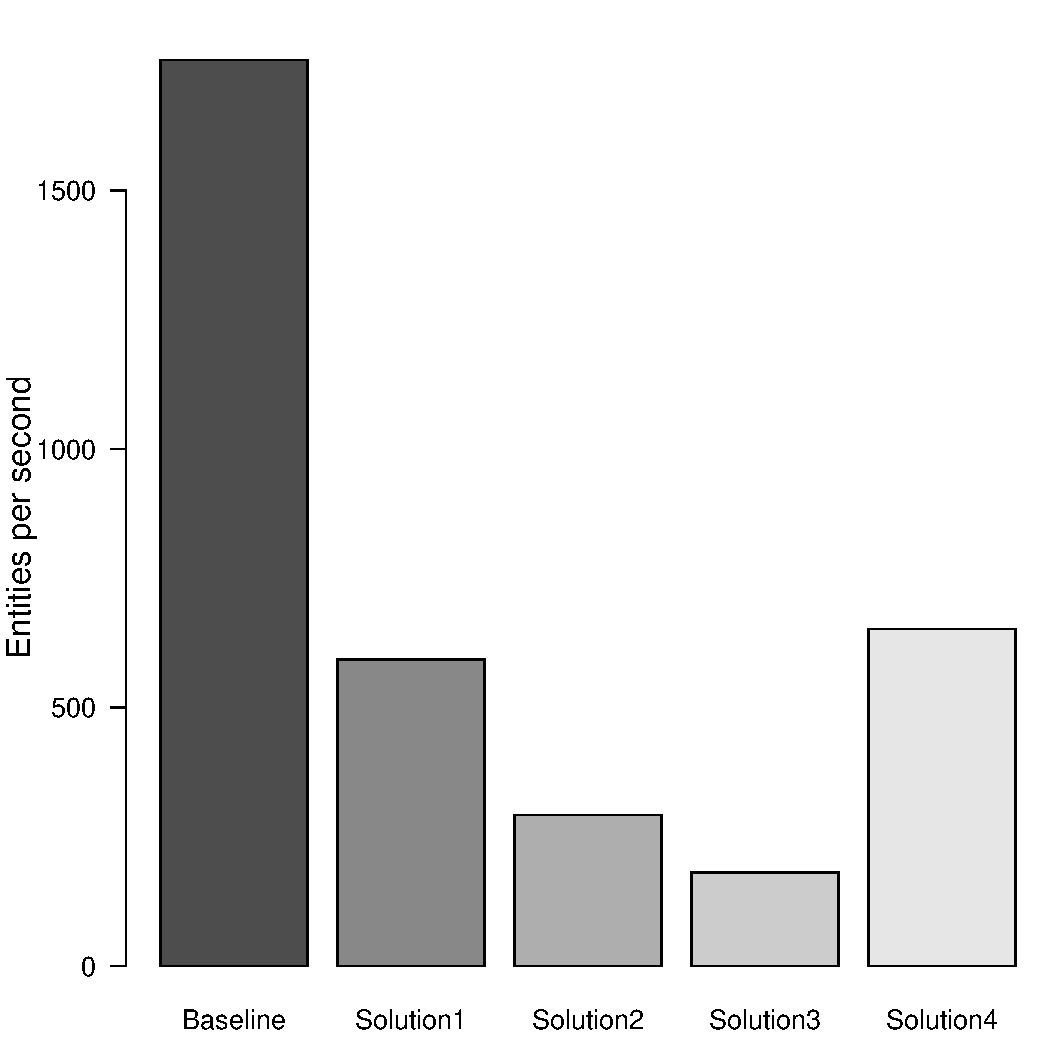
\includegraphics[width=\W]{figure/result/barplot-insert_enrolment-tp.pdf}}
			\caption{Performance inserting enrolments}\label{fres:insert-enrolment}
		\end{figure}